\subsection{Entry criteria}

In order to perform the integration testing of \textbf{PowerEnJoy} the following criteria must be met:
\begin{itemize}
\item The Requirements Analysis and Specification Document (\textbf{RASD}) and the Design Document (\textbf{DD}) must be fully written
\item The components :
\begin{itemize}
\item UserController
\item MapController
\item ReservationController
\item RentController
\item FareController
\item CarController
\item DistributionOptimizer
\item CarRemoteController
\item ClientApp
\end{itemize}
must be developed and unit tested
\item Unit testing must be performed on the \textbf{Model} classes.
\item All the high prioritized faults and bugs found during unit testing must have been fixed
\end{itemize}
\newpage

\subsection{Elements to be integrated}
The elements to be integrated are the components presented in the design document.


\begin{figure}[hp]
\centering
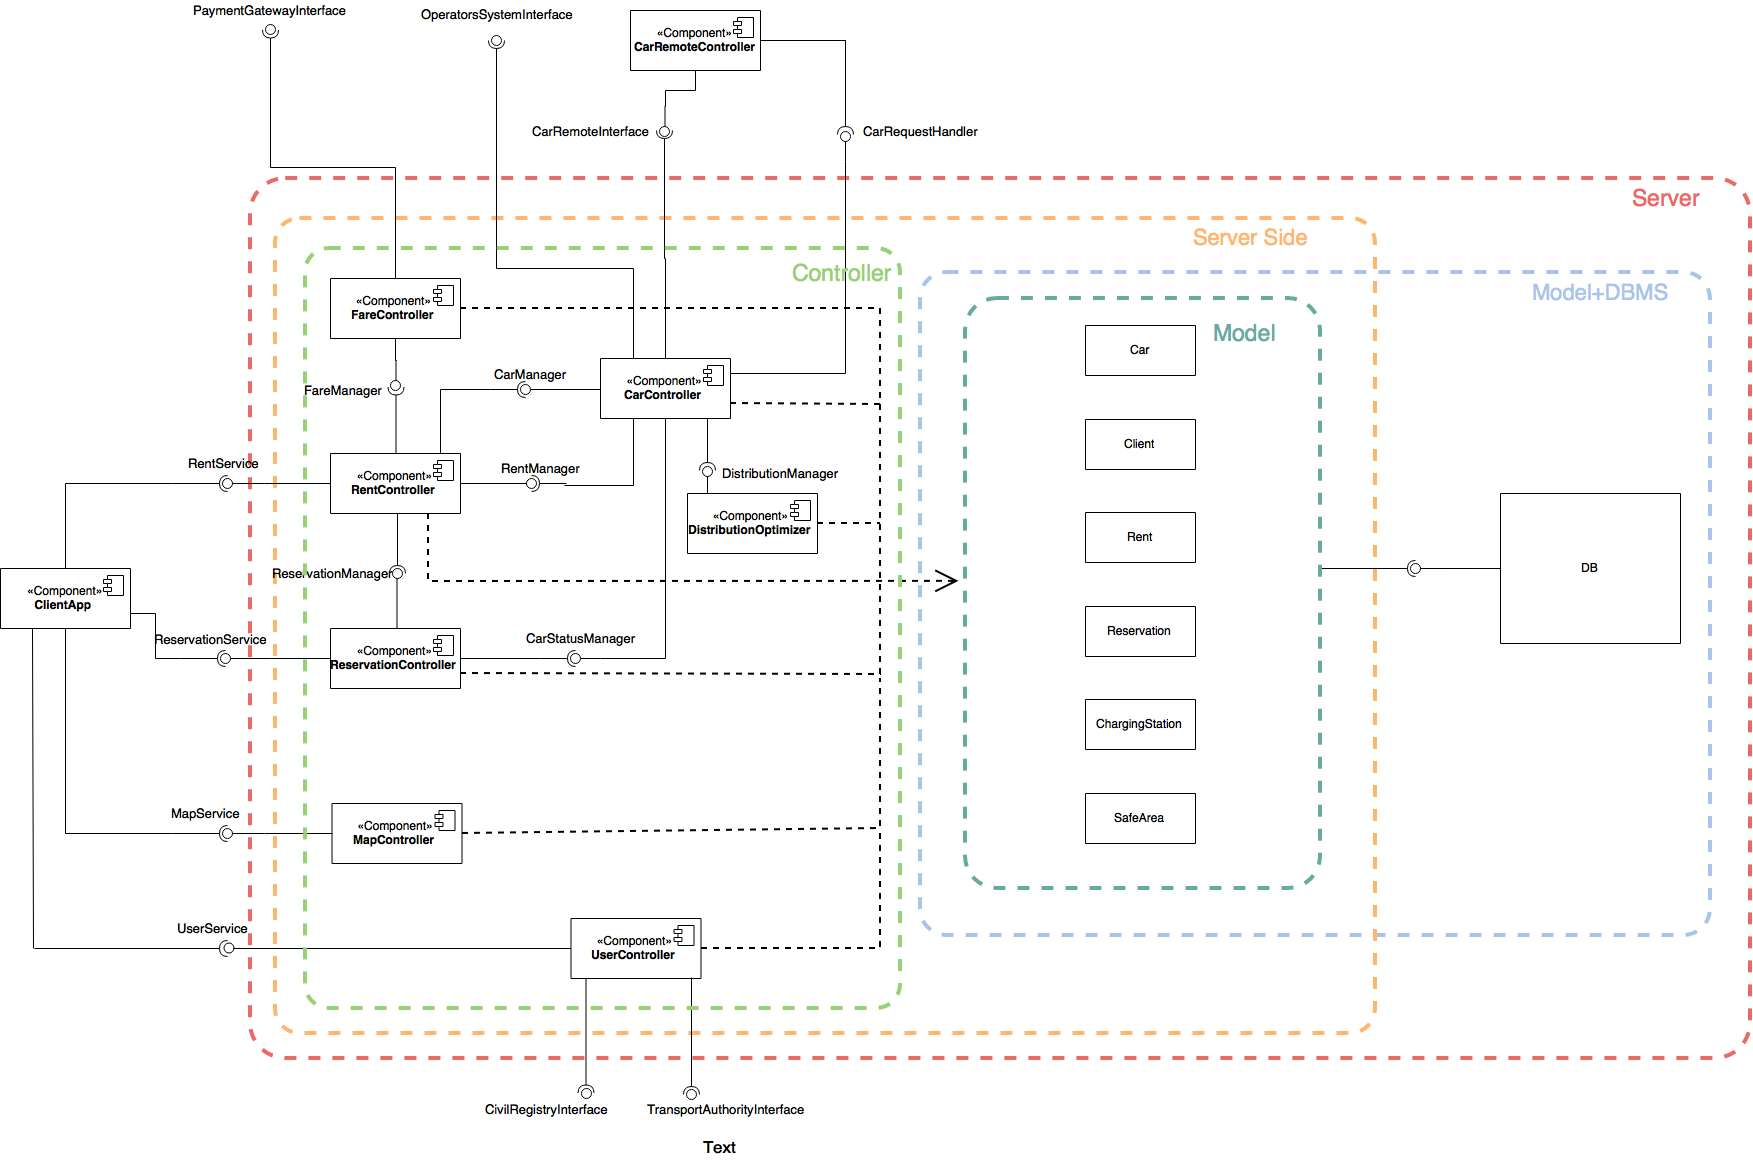
\includegraphics[width=450 pt]{resources/components.png}
\caption{\label{fig:component}Component diagram.}
\end{figure}
Starting from the components of the  diagram above we have identified the following subsystems :

\begin{itemize}
\item \textbf{Controller:} a set of all the controller components on the server side 
\item \textbf{Model:} composed by all the model components on the server side
\item \textbf{Model + DBMS} : composed by the Model and the DBMS 
\item \textbf{Server:} composed by the integration of the Controller with the subsystem Model+DBMS
\end{itemize}

The first integration is between the \textbf{Model} components, however the only interaction between them are getters and setters so we can integrate  all these components without testing them. From now on we will proceed  considering all the model components as an unique component named just \textbf{Model}. The next components to be integrated is the \textbf{DBMS} and the \textbf{Model}, obtaining a subsystem called \textbf{Model+DBMS}. 
Now we have to integrate the \textbf{Controller} components to the \textbf{Model+DBMS} subsystem. Then we can proceed to the integration between the controller components taking into account the yet succeeded integration between each of the \textbf{Controller} modules and the \textbf{Model+DBMS} subsystem. The result of this phase will be the \textbf{Server} subsystem. The next step is to integrate the  remaining standalone components : the \textbf{Client} and the \textbf{CarRemoteController}. In order to accomplish this task will be adopted a functional approach. 
We assume that the teams that will develop the components that use external services will test the external interfaces during the unit testing phase using some tools given by the service provider, so the integration of the external interfaces does not need to be tested again and they will be integrated directly to each component that makes use of them.

\newpage
\subsection{Integration testing strategy}
Due to the complexity of the project and the fact that it is deployed on several hardware devices we are going to use different integration testing approaches.
On a high level we are going to use a \textbf{bottom-up} approach to integrate the subsystems of \textbf{PowerEnjoy}. This incremental approach allows us to detect faster faults and bugs (compared to approaches like "big bang") and to evaluate easily the testing progress.
\begin{figure}[hp]
  \centering
  \includegraphics[width=200 pt]{resources/bottom_up_v2.png}
  \label{fig:bottom_up}
\end{figure}
\\
As written in the "Entry Criteria" all the components of the \textbf{Model} have already been tested and  they don't need integration testing because interacts only with getters and setters. 
Therefore we are going to consider the model as a unique component.\newline
The first step consist on the integration of the \textbf{Model} with the \textbf{DBMS} to test their interaction. \textbf{DBMS} is a commercial component that has already been developed so it can be immediately used in a bottom-up approach without any explicit dependency.
All the components of the \textbf{Controller} subsystem will be first integrated and tested with the \textbf{model} in order to facilitate future integration testing. This can be done separately and independently in order to save time.\newline
To integrate between them the components of the \textbf{Controller} subsystem we are going to 
use a "\textbf{Critical Module First}" approach. Starting from the riskiest and most connected parts will help us to detect bugs as soon as possible, but we will also need to develop some stubs and drivers.
We will start integrating CarController with :
\begin{itemize}
\item ReservationController
\item RentController
\item DistributionOptimizer
\end{itemize}
Also these integrations will be done independently using appropriate stubs and drivers.
We will procede integrating ReservationController with RentController and, after testing,integrating also FareController.

Once the Server has been fully tested, we are going to test the interaction between the three subsystems:
\begin{itemize}
\item ClientApp
\item CarRemoteController
\item Controller + Model + DBMS  (= Server)
\end{itemize}
In this phase a Big Bang approach would be too dispersive and would not guarantee a proper visibility on the functionalities because the system is big and presents complex interactions among his subsystems.
Even if the integration may result more complex, we opt for a \textbf{functional grouping} approach that will require less stubs/drivers and will provide better process visibility.
Portions of the different subsystems interact together to provide the following user-visible functions:
\begin{itemize}
\item Reservation
\item Start Rent
\item Map visualization
\item User Account Management
\item End Rent
\item Damage Report
\item MoneySavingOption Request
\end{itemize}
Another advantage of this approach is that functions can be tested separately and independently by different testing teams in order to speed up the testing process. 


\newpage

\subsection{Sequence of component/function integration}
In the following sub-paragraphs will be explain the order in which the tests between various components and subsystems will be performed. 

\subsubsection{Software integration sequence}

\begin{center}
\begin{tabular*}
{\textwidth}
{l p{8.5cm} l}
\hline
\textbf{ID} & \textbf{Integration Test} & \textbf{Paragraph} \\
\hline
I2T1 & (DBMS + Model) $\rightarrow$ MapController & 3.2\\
I2T2 & (DBMS + Model) $\rightarrow$ UserController & 3.2\\
I2T3 & (DBMS + Model) $\rightarrow$ CarController & 3.2\\
I2T4 & (DBMS + Model) $\rightarrow$ DistributionOptimizer & 3.2\\
I2T5 & (DBMS + Model) $\rightarrow$ ReservationController & 3.2\\
I2T6 & (DBMS + Model) $\rightarrow$ RentController & 3.2\\
I2T7 & (DBMS + Model) $\rightarrow$ FareController & 3.2\\
I3T1 &CarController$\rightarrow$ DistributionOptimizer & 3.3\\
I3T2 &CarController$\rightarrow$ ReservationController & 3.3\\
I3T3 &CarController$\rightarrow$ RentController & 3.3\\
I4T1 &ReservationController$\rightarrow$ RentController & 3.4\\
I5T1 &RentController$\rightarrow$FareController & 3.5\\
\hline
\newline
\newline
\end{tabular*}
\end{center}




As already mentioned, the integration between components follows a mix of bottom-up and critical-module-first approach. In the diagrams below, we focus on the component of the server side. The direction of the arrows indicates the order of integration. 
First of all, the model will be integrated with all controller component, and, for speed up this phase, this can be do in in parallel. This will allow every component to access to data needed for the other tests. On the next step we will integrate the components of the Controller subsystem. We will first integrate CarController with the interacting components: DistributionOptimizer
ReservationController, RentController.
Finally we will perform the  integration between ReservationController and RentController and between RentController and FareController .
The numbers that labels the edges indicate the sequence of integration. Notice that this order coincide with a topological order of the graph.

\begin{figure}[hp]
\centering
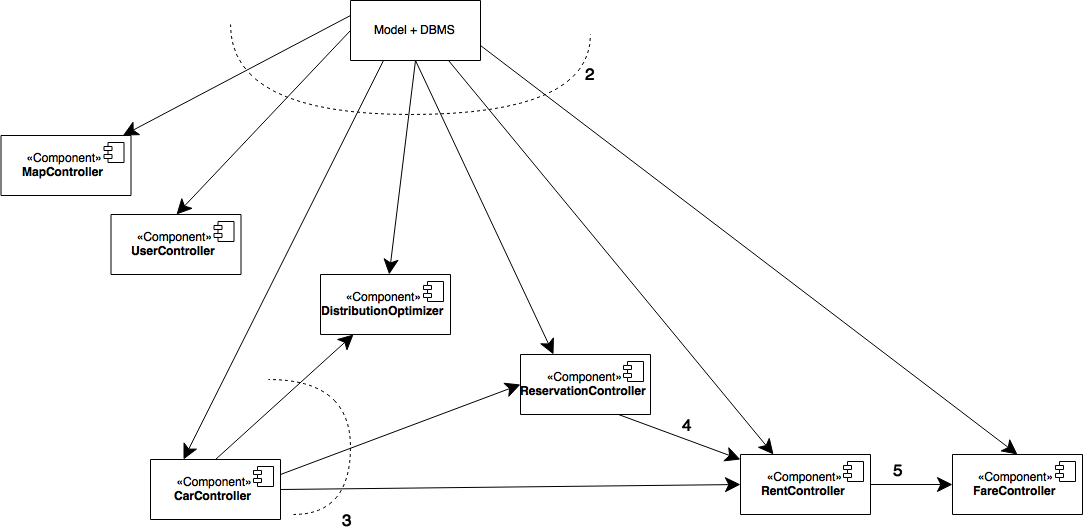
\includegraphics[width=470 pt]{resources/integrationServer.png}
\caption{\label{fig:IntServer}Integration strategy server side.}
\end{figure}


\subsubsection{Subsystem integration sequence}
\begin{center}
\begin{tabular*}
{\textwidth}
{l p{8.5cm} l}
\hline
\textbf{ID} & \textbf{Integration Test} & \textbf{Paragraph} \\
\hline
I1 & DBMS $\rightarrow$ Model & 3.1\\
I2 & (DBMS + Model) $\rightarrow$ Controller & 3.2\\
I6 & Client $\rightarrow$ Server $\rightarrow$ CarController & 3.6\\
\hline
\newline
\newline
\end{tabular*}
\end{center}

PowerEnJoy can be divided into different subsystems, as seen in Design document.
Since that the integration of the subsystems could hide various problems, we have decided to use a functional grouping approach. This strategy allows us to obtain a general view of the desired effects over the full system.

\begin{figure}[hp]
\centering
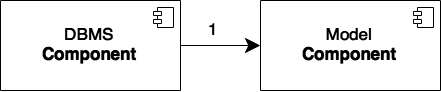
\includegraphics[width=150 pt]{resources/Model_+_DBMS.png}
\caption{\label{fig:Model+DBMS}Model + DBMS subsystem.}
\end{figure}

First of all, to make relevant all the following tests, we must test the integration between \textbf{DBMS} and \textbf{Model} subsystem. Then we focused on the \textbf{Controller} subsystem, as mentioned above, and integrate it with \textbf{DBMS + Model}. After that, we integrate the other server components. This integration has as result the \textbf{Server} subsystem. Finally the last integration will be between the Server subsystem and the remaining components :\textbf{CarController} and \textbf{ClientApp} .




\begin{figure}[hp]
\centering
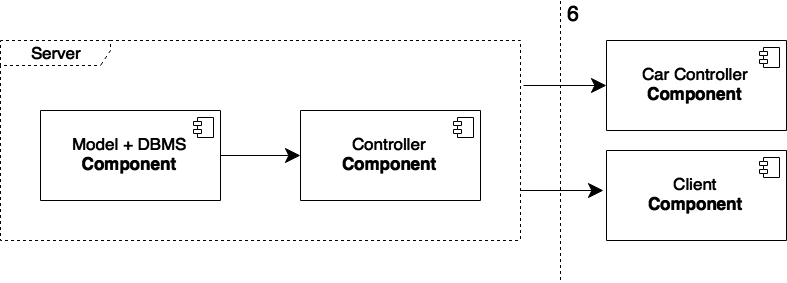
\includegraphics[width=400 pt]{resources/integrationSubSys.png}
\caption{\label{fig:SubSys}Integration strategy subsystem.}
\end{figure}

